\section{WLCG}

As mentioned in section 1, the LHC experiments are designed to
search for rare events with the signal/noise ratio as low
as $10^{-13}$. This Physics requires a study of enormous number of
pp and Pb-Pb collisions resulting in the production of data volumes
of more than 10 PetaBytes per one data taking year. The original
estimates elaborated when the LCG TDR \cite{LHC_TDR} was put together were
about $\sim 15$~PetaBytes (PB) of new data each year which
translates into $\sim 200$ thousands of CPUs/processor cores and
45~PB of disk storage to keep the raw, processed and simulated data.

Nowadays, 200 thousands cores does not sound like much and one can
find them in large computer centers. 50~PB of a disk storage is
however not that common. In any case, at the time the LHC Computing
Grid was launched there was no single site within the LHC community
able to provide such computing power. So, the task of
processing the LHC data has been a distributed computing problem
right from the start.

\subsection{WLCG mission}
%
The Worldwide LHC Computing Grid (WLCG) project was launched in
2002 to provide a global computing infrastructure to store,
distribute and process the data annually generated by the LHC.
It integrates thousands of computers and storage systems
in hundreds of data centers worldwide, see Figure~\ref{fig02} . CERN
itself provides only about 20\% of the resources needed to manage
the LHC data. The rest is provided by the member states' national
computing centers and research network structures supported by
national funding agencies. The aim of the project is the
"collaborative resource sharing" between all the scientists
participating in the LHC experiments, which is the basic concept of
a Computing Grid \cite{GRID}. The infrastructure is managed
and operated by a collaboration between the experiments and the
participating computer centers to make use of the resources no
matter where they are located.

%fig02
\begin{figure}[htb] % h-here, t-top, b-bottom
\centering
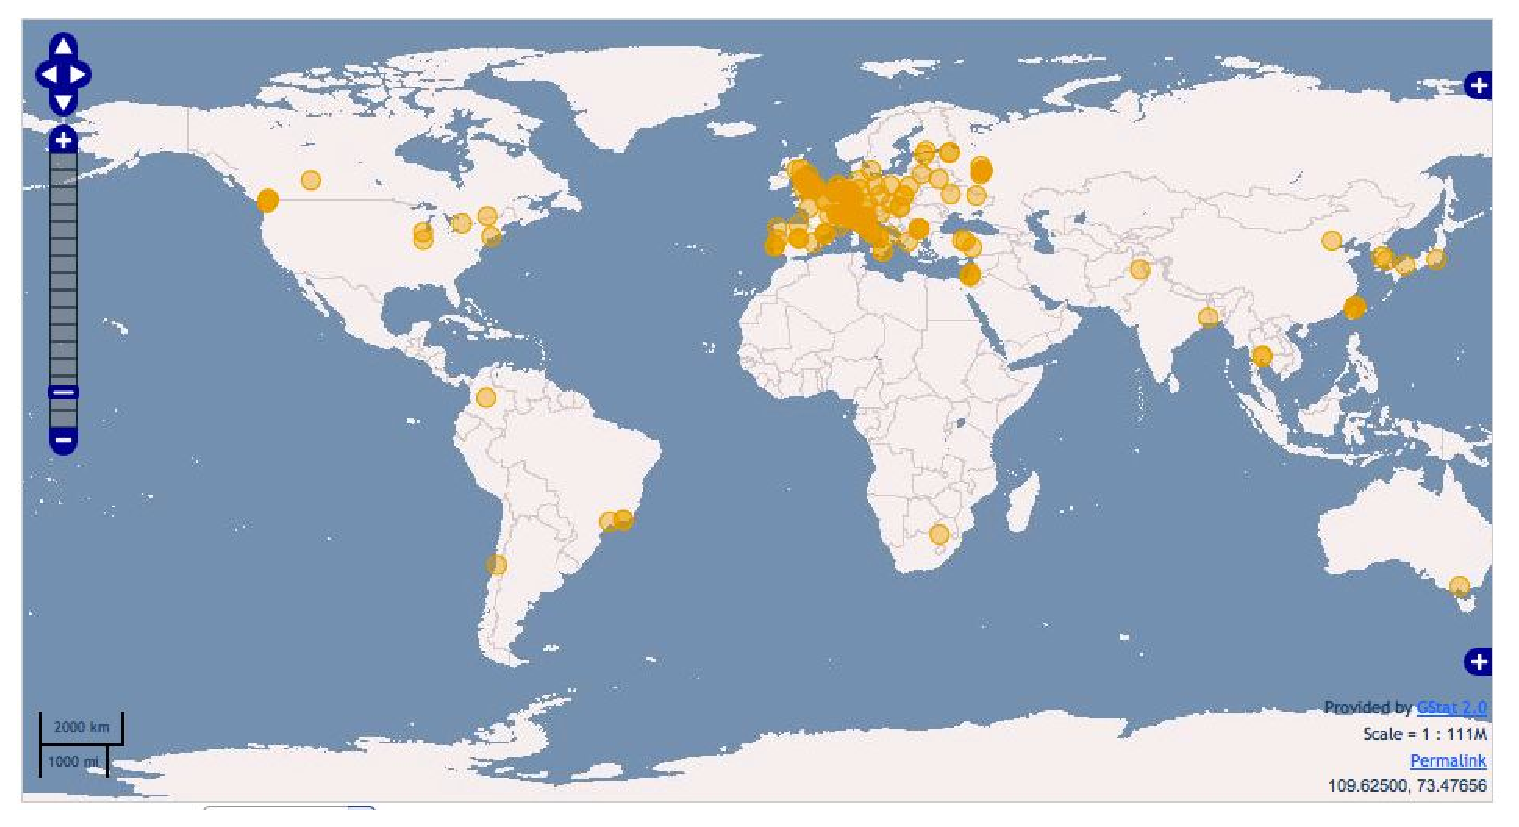
\includegraphics[width=13cm]{fig02.eps} %    ** if .eps don't need extension
\caption{Distribution of WLCG computing centers}\label{fig02}
\end{figure}



The collaboration is truly worldwide: it involves 35 countries on 5
continents and represents 49 funding agencies having signed the WLCG
Memorandum of Understanding on Computing (WLCG MoUC)\cite{MoU}. The
distributed character has also a sociological aspect: even if the contribution 
of the countries depends on  their capabilities, a member of any
institution involved can access and analyze the LHC data from
his/her institute.

Currently, the WLCG integrates over 140 computing sites, more than
250 thousands CPU cores and over 150~PB of disk storage. It is now
the world's largest computing grid: the WLCG operates resources
provided by other collaborating grid projects: either the two main
global grids, EGI \cite{EGI} and OSG \cite{OSG}, or by several regional or
national grids.

\subsection{Hierarchical (Tier) structure, the roles of different
Tier-sites}
%
The WLCG has a hierarchical structure based on the
recommendations of the  MONARC project\cite{MONARC}, see Figure~\ref{fig03}.
The individual participating sites are  classified according to their
resources and level of provided services into several categories
called Tiers. There is one Tier-0 site  which is CERN, then 11 Tier-1
centers, which are large computing centers with thousands of CPUs,
PBs of disk storage, tape storage  systems and 24/7 Grid support
service (Canada: TRIUMF, France: IN2P3, Germany: KIT/FZK,  Italy: INFN,
 Netherlands: NIKHEF/SARA,  Nordic countries: Nordic Datagrid Facility (NDGF), 
Spain: Port d'Informaci\'o
Cient\'ifica (PIC),  Taipei:
ASGC, United Kingdom: GridPP,  USA: Fermilab-CMS and BNL ATLAS).
Then there are currently about 140 Tier-2 sites covering most of the
globe. The system also recognizes Tier-3 centers, which are small
local computing clusters at universities or research institutes.

%fig03
\begin{figure}[htb] % h-here, t-top, b-bottom
\centering
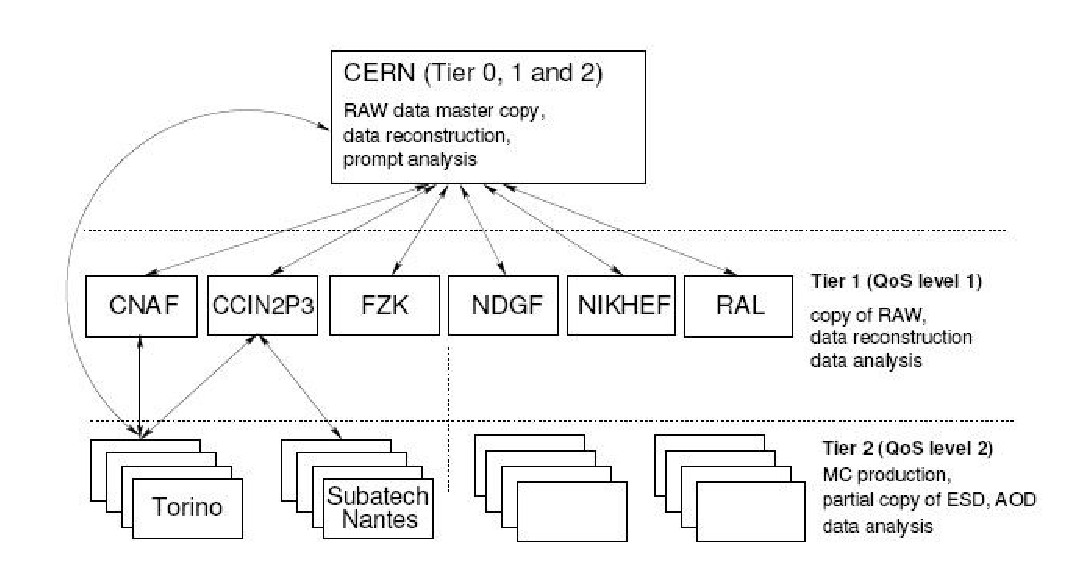
\includegraphics[width=13cm]{fig03.eps} %    ** if .eps don't need extension
\caption{Schema of the hierarchical Tier-like structure of
WLCG}\label{fig03}
\end{figure}




The raw data recorded by the LHC experiments  is shipped
first to the CERN Computing Center (CC) through dedicated links.
CERN Tier-0 accepts data at average of 2.6~GBytes(GB)/s with peaks
up to 11 GB/s. At CERN, the data is archived in the CERN tape system
CASTOR \cite{castor} and goes through the first level of processing - the
first pass of reconstruction. The raw data is also replicated to the
Tier-1 centers, so there are always 2 copies of the raw data files.
CERN serves data at average of 7 GB/s with peaks up to 25 GB/s \cite{TERENA}.
The Tier-0 writes on average 2~PB of data per month to tape in pp
running, and double that in the 1 month of Pb-Pb collisions, (cf.
Figures~\ref{fig04},\ref{fig05}).


%fig04
\begin{figure}[htb] % h-here, t-top, b-bottom
\centering
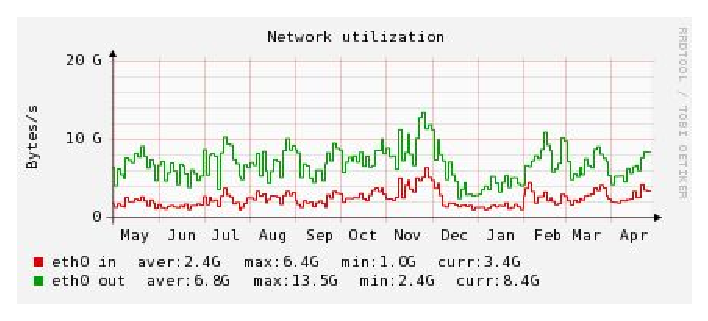
\includegraphics[width=13cm]{fig04.eps} %    ** if .eps don't need extension
\caption{CERN Tier-0 Disk Servers (GB/s), 2010/2011}\label{fig04}
\end{figure}



%fig05
\begin{figure}[htb] % h-here, t-top, b-bottom
\centering
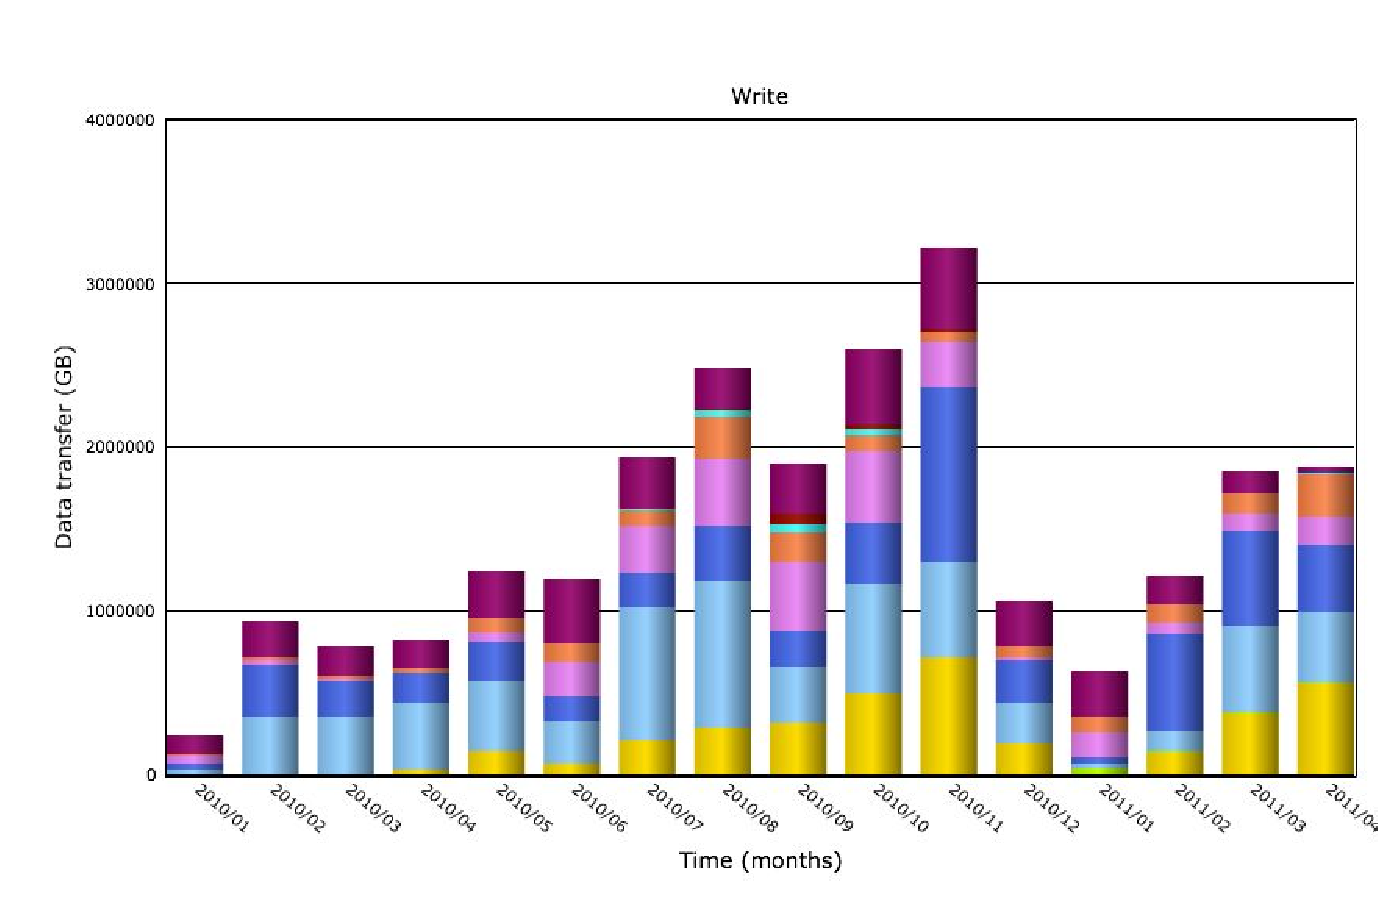
\includegraphics[width=13cm]{fig05.eps} %    ** if .eps don't need extension
\caption{Data written to tape at the CERN Tier-0
(GB/month)}\label{fig05}
\end{figure}


At Tier-1 centers, the raw data replicas are permanently stored as
mentioned before and several passes of the data re-processing are
performed. This multiple-stage data re-processing is performed using
methods to detect interesting events through the processing
algorithms, as well as improvements in detector calibration, which
are in continuous evolution and development. Also, the scheduled
analysis productions as well as some of the end user analysis jobs
are performed at Tier-1s.

Tier-2 centers  (more than 130 in the WLCG, integrated within 68
Tier-2 federations) are supposed to process simulation (Monte Carlo
simulations of the collision events in the LHC detectors) and
end-user analysis jobs. The load of simulations needed to correctly
interpret the LHC data is quite sizeable, close to the raw data
volume. The number of end users regularly using the WLCG
infrastructure to perform analysis is larger than expected in the
beginning of the LCG project, it varies from about 250 to 800 people
depending on the experiment. This is certainly also a result of the
experiments' effort to hide the complexity of the Grid from the
users and make the usage as simple as possible. Tier-2 sites deliver
more than 50\% of the total CPU power within the WLCG, see
Figure~\ref{fig06}.

%fig06
\begin{figure}[htb] % h-here, t-top, b-bottom
\centering
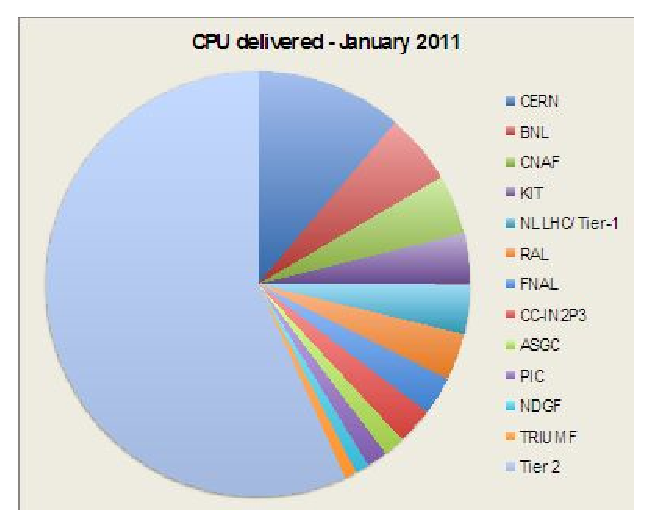
\includegraphics[width=13cm]{fig06.eps} %    ** if .eps don't need extension
\caption{CPU resources in WLCG, January 2011. More than 50\% was
delivered by Tier-2s.}\label{fig06}
\end{figure}



\subsection{Network}
%
The sustainable operation of the data storing and processing
machinery would not be possible without a reliable network
infrastructure. In the beginning of the WLCG project there were
worries that the infrastructure would not be able to transfer the
data fast enough. The original estimates of the needed rate were
about 1.3~GB/s from CERN to external Tiers. After the years spent
with building the backbone of the WLCG network, CERN
is able to reach rates about 5~GB/s to Tier-1s, see
Figure~\ref{fig07}.

%fig07
\begin{figure}[htb] % h-here, t-top, b-bottom
\centering
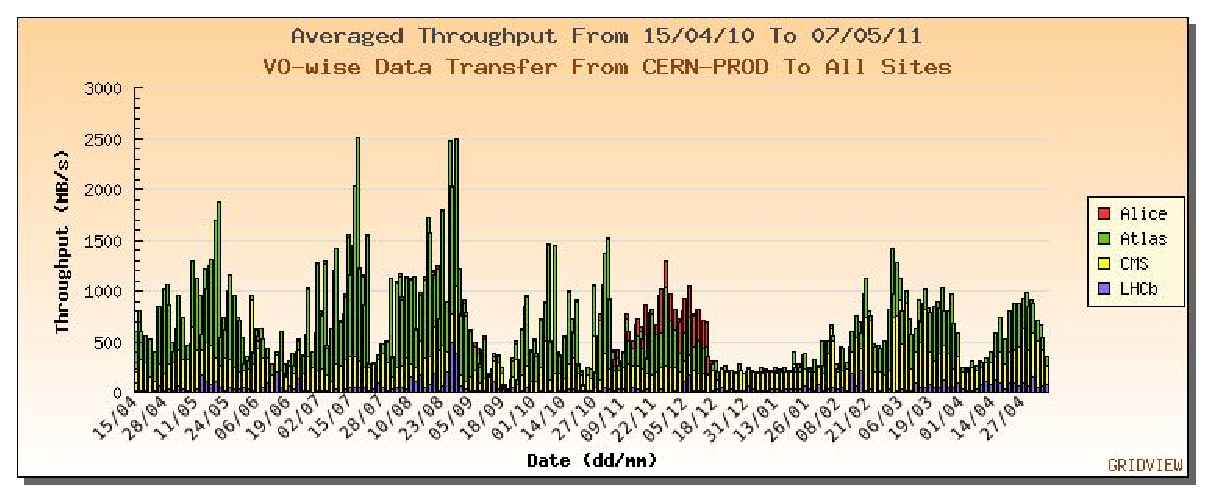
\includegraphics[width=13cm]{fig07.eps} %    ** if .eps don't need extension
\caption{Average throughput from CERN to all Tiers}\label{fig07}
\end{figure}


The WLCG networking relies on the Optical Private Network (OPN)
backbone \cite{OPN}, see Figure~\ref{fig08}, which is composed of dedicated
connections between CERN Tier-0 and each of the Tier1s, with the
capacity of 10~Gbit/s each. The original connections proliferated
into duplicates or backroutes making the system considerably
reliable. The OPN is then interconnected with national network
infrastructures like the GEANT \cite{GEANT} in Europe or the US-LHCNet \cite{USLHCNET}
and all the National Research and Education Networks (NRENs) in
other countries.

%fig08
\begin{figure}[htb] % h-here, t-top, b-bottom
\centering
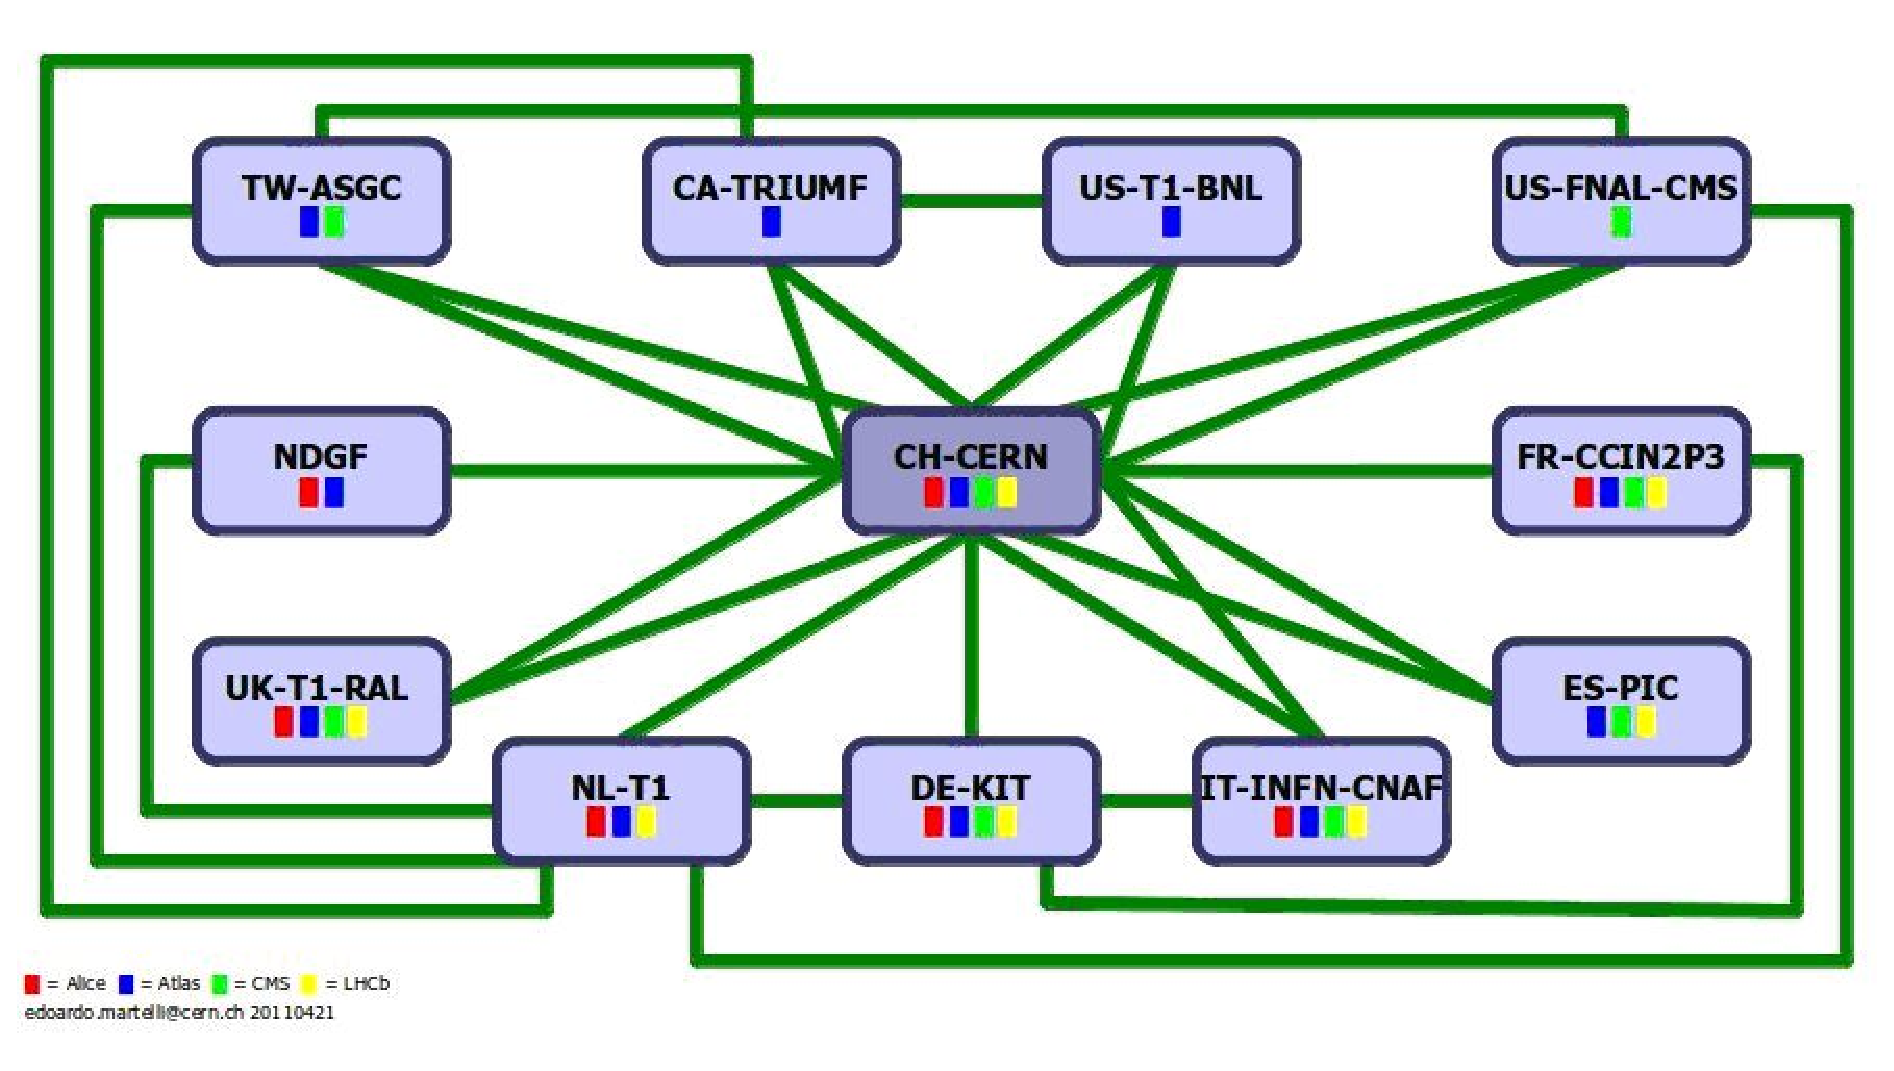
\includegraphics[width=13cm]{fig08.eps} %    ** if .eps don't need extension
\caption{LHCOPN}\label{fig08}
\end{figure}


There exists a concept of so-called LHCONE \cite{LHCONE}, which should enable
a good connectivity of Tier-2s and Tier-3s to the Tier-1s without
overloading the general purpose network links. It will extend and
complete the existing OPN infrastructure to increase the
interoperability of all the WLCG sites.

\subsection{Data and Service challenges}
%
As we will describe in section~6, the WLCG data management
worked flawlessly when the real data started
to flow from the detectors in the end of 2009. This was not just
a happy coincidence. There were over 6 years of continuous testing
of the infrastructure performance. There was a number of independent
experiments' so-called Data Challenges which started in 2004, when
the "artificial raw" data was generated in the Monte Carlo
productions and then processed and managed as if it was the real raw
data. More over,  there was a series of WLCG Service Challenges also
starting in 2004, with the aim to demonstrate WLCG services aspects:
data management, scaling of job workloads, security incidents,
interoperability, support processes and all was topped with data
transfers exercise lasting for weeks. The last test was the Service
Challenge STEP'09 including all experiments and testing full
computing models. Also, the cosmic data taking which started in 2008
has checked the performance of the data processing chain on a
smaller scale.

Currently, whether the data taking is going on or not, the network,
especially the OPN, and the sites are under continuous checking:
there  are automatically generated test jobs periodically sent over
the infrastructure to test the availability and functioning of the
network and on-site services.

\subsection{Concluding remarks}
%
The WLCG integrates and operates resources distributed all over the
world and its task is to make all these resources accessible and
usable for the LHC experiments to distribute, archive and process
the data produced by the LHC. This task is done using a specialized
software called ``middleware'' because it sits between the operating
systems of the computers at the WLCG sites and the Physics
applications software used for the reconstruction, analysis and
simulation of the LHC data (or any other application software
layer). The middleware is a collection of protocols, agents and
programs/services which we describe in the following section.

